\documentclass[tikz,border=2pt]{standalone}
\usepackage{amsmath,amssymb}
\usepackage{tikz}
\usetikzlibrary{arrows.meta}

\begin{document}
% Differentiating twice: each first-order partial can be differentiated again w.r.t. each
% variable, giving the four second-order partials of f(x,y), which fill the Hessian.
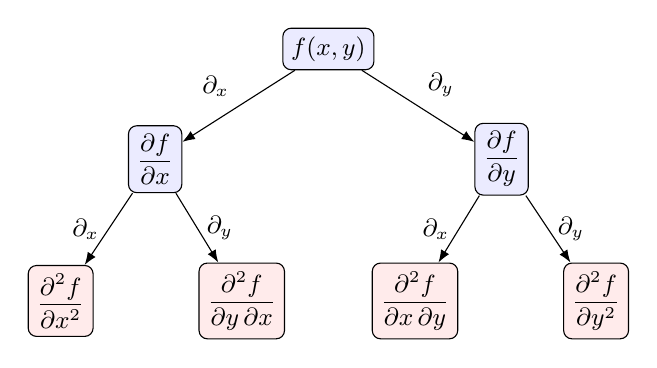
\begin{tikzpicture}[every node/.style={font=\small}, >={Latex[length=1.6mm]}, lvl/.style={draw, rounded corners=3pt, fill=blue!8, inner sep=3pt}]
	\node[lvl] (f) at (0,0) {$f(x,y)$};
	\node[lvl] (x) at (-2.2,-1.4) {$\dfrac{\partial f}{\partial x}$};
	\node[lvl] (y) at (2.2,-1.4) {$\dfrac{\partial f}{\partial y}$};
	\node[lvl, fill=red!8] (xx) at (-3.4,-3.2) {$\dfrac{\partial^2f}{\partial x^2}$};
	\node[lvl, fill=red!8] (xy) at (-1.1,-3.2) {$\dfrac{\partial^2f}{\partial y\,\partial x}$};
	\node[lvl, fill=red!8] (yx) at (1.1,-3.2) {$\dfrac{\partial^2f}{\partial x\,\partial y}$};
	\node[lvl, fill=red!8] (yy) at (3.4,-3.2) {$\dfrac{\partial^2f}{\partial y^2}$};
	\draw[->] (f) -- (x) node[midway, above left] {$\partial_x$};
	\draw[->] (f) -- (y) node[midway, above right] {$\partial_y$};
	\draw[->] (x) -- (xx) node[midway, left] {$\partial_x$};
	\draw[->] (x) -- (xy) node[midway, right] {$\partial_y$};
	\draw[->] (y) -- (yx) node[midway, left] {$\partial_x$};
	\draw[->] (y) -- (yy) node[midway, right] {$\partial_y$};
\end{tikzpicture}
\end{document}
